\documentclass{article}

\usepackage{amsmath}
\usepackage{amssymb}
\usepackage{mathbbol}
\usepackage{algorithmicx}
\usepackage{algpseudocode}
\usepackage{cite}
\usepackage{flushend}
\usepackage{graphicx}
\usepackage{graphics}
\usepackage{url}
\usepackage[table]{xcolor}
\usepackage{xspace}
\usepackage[T2A]{fontenc}

\usepackage{algorithm}
\usepackage[english]{babel}

\usepackage[utf8]{inputenc}

\newcommand{\OM}{\textsc{OneMax}\xspace}
 \newcommand{\J}{\textsc{Jump}\xspace}
\newcommand{\LB}{\textsc{LeftBridge}\xspace}
\newcommand{\RB}{\textsc{RightBridge}\xspace}
\newcommand{\EARL}{\textsc{EA+RL}\xspace}
\newcommand{\RLS}{\textsc{RLS}\xspace}
\newcommand{\OMZM}{\textsc{OneMax+ZeroMax}\xspace}
\newcommand{\XdK}{\textsc{XdivK}\xspace}

%\allowdisplaybreaks

\begin{document}

\section{Problem statement}

We consider simple $(1 + 1)$-ES. It has only one individual in population and on each iteration it creates new individual by mutating each bit of the current individual with probability of $\frac{\lambda}{n}$, where $\lambda$ is a mutation rate that is a fixed constant during an algorithm run. It accepts the new individual if and only if its fitness value is not worse then the fitness value of the current individual.

At first we considered \XdK function. But it seemed too complicated, so we simplified it to the following function $F$ that has some parameter $k$, as \XdK does:

\begin{align*}
  F(x) =
  \begin{cases}
    \OM(x), \text{ if } \OM(x) \le n - k \\
    n - k, \text{ if } n - k < \OM(x) < n \\
    n, \text{ if } \OM(x) = n \\
  \end{cases}
\end{align*}

Our aim is to find the optimal value of the mutation rate $\lambda$ that minimizes the expected runtime of the algorithm. If we reach our goal, we will be able to compare it the Fast Genetic Algorithm.

\section{First subproblem}
As passing over the plateau in the end of optimization process requires most time (at least $\Omega(n^2)$ for $k \ge 2$, while reaching the plateau requires only $O(n \log n)$), we are most interested in finding optimal $\lambda$ for passing the plateau. Attempts to find it that have been made by this moment are described in this document

\section{Notation}

We consider a Markov chain that illustrates the behaviour of the considered algorithm on the plateau of the function $F$. It has $k + 1$ states that are numbered from $0$ to $k - 1$. If the algorithm is in state $i$, then the current individual has exactly $n - k + i$ one-bits in it. 

By $p_i^j$ we imply the probability that algorithm that is in state $i$ will get to state $j$ on the next iteration.

The exact value of this probabilities is quite complicated:

\begin{align*}
  p_i^j = \begin{cases}
    \sum\limits_{m = 0}^{k - j} \binom{k - i}{j - i + m} \binom{n - k + i}{m} \left(\frac{\lambda}{n}\right)^{j - i + 2m} \left(1 - \frac{\lambda}{n}\right)^{n - j + i - 2m}, \text{ if } j > i \\
      \sum\limits_{m = 0}^{k - i} \binom{k - i}{m} \binom{n - k + i}{i - j + m} \left(\frac{\lambda}{n}\right)^{i - j + 2m} \left(1 - \frac{\lambda}{n}\right)^{n - i + j - 2m}, \text{ if } j < i \\
      1 - \sum\limits_{m = 0, m \ne i}^{k + 1} p_i^m, \text{ if } j = i \\
  \end{cases}
\end{align*}

However this sums for $i \ne j$ without their first summand are much smaller then their first summand. Empirically it was shown that if we assume that every mutation flips only ones or only zeros, then the expected time of the algorithm does not change, so for first results we can perform our analysis with simplified probabilities that contain only their first summand. You can see the comparison of the expected runtimes with simplified and wit original probabilities for $k = 10$ and $n = 100$ in Fig.~\ref{plot_simpl}.

\begin{figure}[t]
 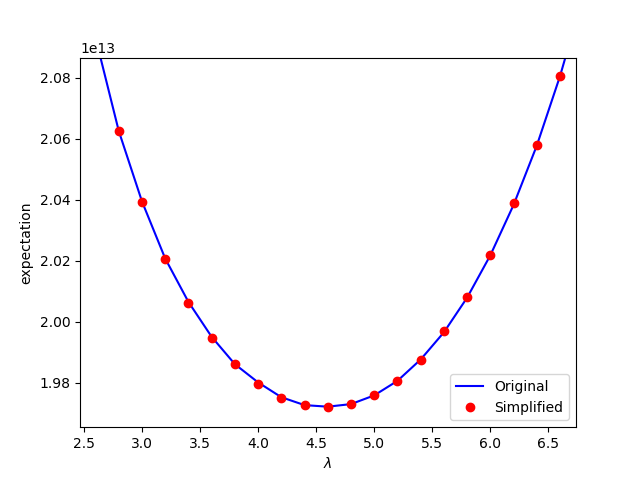
\includegraphics[width=0.8\textwidth]{pic/simplified_probs.png}
 \caption{Comparison of runtimes with original and simplified probabilities for $n = 100$ and $k = 10$.
 \label{plot_simpl}}
\end{figure}


\section{Bruteforce}

First, we tried just to write a system  of linear equations for expected number of iterations which algorithm requires to get to the state $k$ for each state of the Markov chain. We got this system from following ideas. First let us define $E_i$ -- the expected number of iterations that algorithm needs to get to state $k$ from state $i$. Then if algorithm is in state $i$ it would definitely make at least one step and then it will expectedly need $E_j$ more iterations, where $j$ is a new state of the algorithm after the performed state. So for every $i \in [0; k-1]$ we got the following equation:

\begin{align*}
 E_i = 1 + \sum\limits_{j = 0}^{k - 1} p_i^j E_j.
\end{align*}

Notice that the sum does not include summand $p_i^k E_k$, as $E_k = 0$.

So we have $k$ linear equations and $k$ unknown expectations. After some transformations we got a system that can be represented by the following matrix:

$$
 \left(
  \begin{array}{ccccc|c}
   1 - p_0^0 & -p_0^1 & -p_0^2 & \dots & -p_0^{k - 1} & 1 \\
   -p_1^0 & 1 - p_1^1 & -p_1^2 & \dots & -p_1^{k - 1} & 1 \\
   -p_2^0 & -p_2^1 & 1 - p_2^2 & \dots & -p_2^{k - 1} & 1 \\
   \vdots & \vdots & \vdots & \ddots & \vdots & \vdots \\
   -p_{k - 1}^0 & -p_{k - 1}^1 & -p_{k - 1}^2 & \dots & 1 - p_{k - 1}^{k - 1} & 1 \\
  \end{array}
 \right)
$$

Next we will define matrix $P = (p_i^j)$. Then the previous system may be written as $(I - P)E = 1$, where $I$ is an identity matrix, $E$ - vector of unknown expectations and $1$ is a vector of all ones. Our aim is to find $E = (I - P)^{-1} 1$, however, it's not a simple task.

I found solutions of this system for $k = 2$ and for $k = 3$, however even the second one was too complicated. 

Here is solution for $k = 2$:

\begin{align*}
 E_0 &= \frac{p_0^1 + p_1^0 + p_1^2}{(p_1^0 + p_1^2)(p_0^1 + p_0^2) - p_0^1 p_1^0} \\
 E_1 &= \frac{p_0^1 + p_1^0 + p_0^2}{(p_1^0 + p_1^2)(p_0^1 + p_0^2) - p_0^1 p_1^0} 
\end{align*}

If we substitute all $p_i^j$ with its values, we will get:

$$E_0 \sim E_1 \sim \frac{n^2 e^\lambda}{\lambda(2 + \lambda)}$$

It is easy to see then that the least asymptotical value of the expected runtime is provided by $\lambda = \sqrt{2}$.

Here is solution for $k = 3$ (only for $E_2$, as $E_1$ and $E_0$ are presented by similar complicated expressions:

\begin{tabular}{cc}
 $E_2 =$ & \begin{tabular}{p{12cm}}$((p_2^0 + p_2^1 + p_2^3)(p_0^1 + p_0^2 + p_0^3) - p_0^2 p_2^0)((p_1^0 + p_1^2 + p_2^3)(p_0^1 + p_0^2 + p_0^3) - p_0^1 p_1^0) - (p_1^2(p_0^1 + p_0^2 + p_0^3) + p_0^2 p_1^0)(p_2^1(p_0^1 + p_0^2 + p_0^3) + p_0^1 p_2^0)$ \tabularnewline\hline
$(p_1^0 + p_0^1 + p_0^2 + p_0^3)(p_0^1 p_2^1 + p_1^2 (p_0^1 + p_0^2 + p_0^3)) + (p_2^0 + p_0^1 + p_0^2 + p_0^3)((p_1^0 + p_1^2 + p_2^3)(p_0^1 + p_0^2 + p_0^3) - p_0^1 p_1^0)$\tabularnewline
\end{tabular}
\end{tabular}

So, we have $E_0 \sim E_1 \sim E_2 \sim \frac{n^3 e^\lambda}{\lambda^3 + 3\lambda^2 + 6\lambda}$

Optimal value of $\lambda$ will be $\lambda = \sqrt[3]{6}.$

\section{Assumption after the bruteforce}

This section tells only about some thoughts that were and were not approved by experiments.

It would be beautiful, if optimal value of $\lambda$ was $\sqrt[k]{k!}$ for every $k$. Empirical results has shown that this is likely to be true for at least $k \le 10$ (for lager $k$ the precision of float numbers is not enough).

Most likely expression for all $E_i$ should look like $n^k / f_k(\lambda)$ and $f_k(\lambda)$ should reach its maximum in $\lambda = \sqrt[k]{k!}$ so that our assumption was true. For example, it could be $$\int e^{-\lambda} (\lambda^k - k!)d\lambda = k! e^{-\lambda} \sum\limits_{i = 1}^k \frac{\lambda^i}{i!}.$$

It asymptotically matches our results for $k = 2$ and $k = 3$ (Fig.~\ref{asmp2}) but it totally differs for $k = 10$ (Fig.\ref{asmp10}).

\begin{figure}
 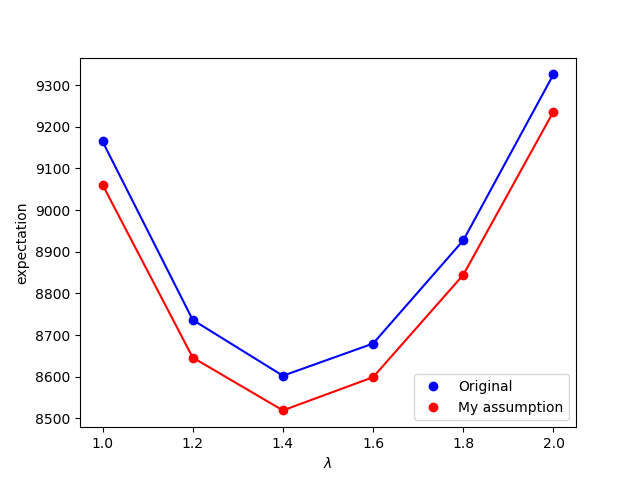
\includegraphics[width=0.8\textwidth]{pic/my_assumption_k2.png}
 \caption{Exact expected runtime and assumed expected runtime for $n = 100 and k = 2$
 \label{asmp2}}
\end{figure}

\begin{figure}
 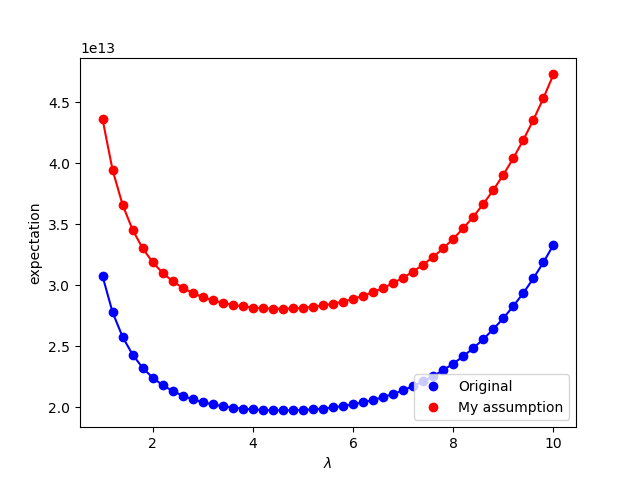
\includegraphics[width=0.8\textwidth]{pic/my_assumption_k10.png}
 \caption{Exact expected runtime and assumed expected runtime for $n = 100 and k = 10$
 \label{asmp10}}
\end{figure}

\section{Simlifiying the sytem}

Benjamin made an assumption that we can simplify our system by assuming that every transition from state $i$ to state $j < i$ goes directly to state $0$. I checked this assumption empirically and it showed that this minor changes shift optimal value of $\lambda$ (Fig.~\ref{doerr})

\begin{figure}
 \label{doerr}
 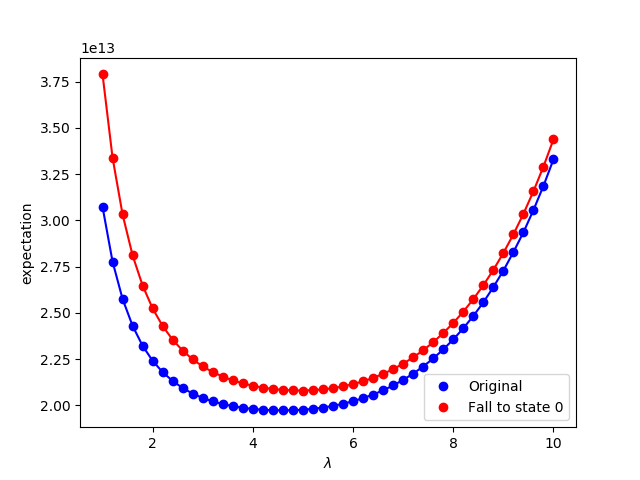
\includegraphics[width=0.8\textwidth]{pic/doerr.png}
 \caption{Exact expected runtimes for original problem and for modified problem, where every fall leads to state $0$
 \label{doerr}}
\end{figure}


\section{Trying to apply Drift theorems}

Next, there was a thought that we can apply drift theorems to our problem. First, I had to decide, what drift should I use, and additive drift seemed most suitable here. So we could define potential function $\Phi_k(state)$ such that $\Phi_k(0)  = 1$ and $\Phi_k(k) = 0$, so we only need to define $(k - 1$ more values of it. However, it turned to be a problem that is harder than finding expectations itself. It could be done by solving a new system of linear equations, that requires that drift from all states must be the same, but this system looks even harder:

$$
 \left(
  \begin{array}{ccccc|c}
   - p_0^1 & -p_0^2 & \dots & -p_0^{k - 1} & -1 & p_0^0 - 1 \\
   1 -p_1^1 & - p_1^2 & \dots & -p_1^{k - 1} & -1 & p_1^0 \\
   -p_2^1 & 1 -p_2^2 & \dots & -p_2^{k - 1} & -1 & p_2^0 \\
   \vdots & \vdots & \ddots & \vdots & \vdots & \vdots \\
   -p_{k - 1}^1 & -p_{k - 1}^2 & \dots & 1 - p_{k - 1}^{k - 1} & -1 & p_{k - 1}^0 \\
  \end{array}
 \right)
$$

So I had to leave this idea.

\section{Finding stable distribution}

Let's consider probability to by in the state $s$ on iteration $i$ -- $q_s(i)$. We define the stable distribution as a vector $\{\lim\limits_{i \to \infty}  q_s(i) \}_{s = 0}^{k}$, if all the limits exist. Obviously, as we always have nonzero probability to get to the state $k$ but we never leave it, this stable distribution will be a vector $(0, 0, \dots 0, 1)$. 

So let us define $p_s(i)$ as a probability to be in state $s$ on iteration $i$ with condition that algorithm has not ended before iteration $i$. So we define the conditional distribution on iteration $i$ as a vector $X_i = \{p_s(i)\}_{s = 0}^{k - 1}$ and we define the stable conditional distribution as a vector $X = \{\lim\limits_{i \to \infty}  p_s(i) \}_{s = 0}^{k - 1}$.

Now we can actually write the expected runtime of the algorithm, if we have an initial distribution $X_0$:

$$E = \sum\limits_{i = 0}^{+\infty} i \cdot p_\text{get}(i) \cdot p_\text{end}(i)$$

Here $p_\text{end}(i)$ is a probability to get to state $k$ on iteration $i$ with condition that the algorithm have not done it before. It can be written as $$\sum\limits_{s = 0}^{k - 1} p_s(i) \cdot p_s^k.$$
$p_\text{get}(i)$ is a probability that algorithm does not get to state $k$ till iteration $i$. It can be found as $$\prod\limits_{j = 0}^{i - 1} (1 - p_\text{end}(j)).$$

How does it help us?

My assumption is following: there exists some number $d$ such that $\sum\limits_{i = 0}^{d} i \cdot p_\text{get}(i) \cdot p_\text{end}(i)$ is $o(E)$ and at the same time $X_i$ is really close to $X$ for $i > d$. It will give us a right to consider $p_\text{end}(i)$ as some constant and $p_\text{get}$ as a geometric sequence.

The first step to find this number $d$ is to find the stable conditional distribution. It exists, as we get $X_{i + 1} = P_\text{cond}^T X_i$ ($P^T$ is a transponded conditional transition matrix) and $P_\text{cond}^T$ is a linear operator that reflects the set of all vectors $X$ such that $X[i] \ge 0 \forall i$ and $\sum X[i] = 1$  to itself. $P_\text{cond}^T$ can be represented by matrix:

$$
 \left(
  \begin{array}{ccccc|c}
   \frac{p_0^0}{1 - p_0^{k}} & \frac{p_1^0}{1 - p_1^{k}} & \frac{p_2^0}{1 - p_2^{k}} & \dots & \frac{p_{k - 1}^0}{1 - p_{k - 1}^{k}} & 0 \\
   \frac{p_0^1}{1 - p_0^{k}} & \frac{p_1^1}{1 - p_1^{k}} & \frac{p_2^1}{1 - p_2^{k}} & \dots & \frac{p_{k - 1}^1}{1 - p_{k - 1}^{k}} & 0 \\
   \frac{p_0^2}{1 - p_0^{k}} & \frac{p_1^2}{1 - p_1^{k}} & \frac{p_2^2}{1 - p_2^{k}} & \dots & \frac{p_{k - 1}^2}{1 - p_{k - 1}^{k}} & 0 \\
   \vdots & \vdots & \vdots & \ddots & \vdots & \vdots \\
   \frac{p_0^{k - 1}}{1 - p_0^{k}} & \frac{p_1^{k - 1}}{1 - p_1^{k}} & \frac{p_2^{k - 1}}{1 - p_2^{k}} & \dots & \frac{p_{k - 1}^{k - 1}}{1 - p_{k - 1}^{k}} & 0 \\
  \end{array}
 \right)
$$

To find stable distribution we need to solve equation $X = P_\text{cond}^T X$. Actually it is a system of linear equations again. However, it has multiple solutions, as it's strings are linearly dependent: their sum gives us a vector of all zeros. But fortunately only one solution will satisfy the constraint that $\sum X[i] = 1$. So, actually we have one extra equation in this system.

How to find it's solution?

The system is still complicated (as well as the system for expected runtimes)
However, it is easier to solve by hands for small values of $k$.

For $k = 2$ $X = (1 - \frac{2}{n + 1} + o(1/n), \frac{2}{n + 1} + o(1/n)).$

For $k = 3$ $X = (1 - \frac{3}{n + 1} + o(1/n), \frac{3}{n + 1} + o(1/n), \frac{6}{n^2} + o(1/n^2)).$

It's not enough information to make any assumptions about $X$, but I feel optimistic about this direction of research. System for $k = 4$ is quite bulky, but still possible to be solved. I hope, it will give us any hints about the $X$.

\end{document}
